\section{Views}

% Document architecture using your selected views (at least logical, process 
% and development) through diagrams and supporting/explaining text. 

\subsection{Logical View}
\label{logicalview}

Below is a class diagram for our program. We split the Client and the Server parts, to better show how the classes interact on their respective sides. For information of how the client and server communicate, please take a look at the the Component Diagram \ref{developmentview}.

As you can see, the Client side classes are only Graphical User Interface classes, that is, they belong to the View part of MVC. The actions performed by the player in the GameGUI will trigger events handled on the server. The GameGUI will then in turn display the consequences.

The Server is responsible for the game logic and consistency. The Game class holds most of the game logic, including the ``run loop'' which keeps the game going and changes player after each iteration. After each turn, it saves the game state to the database so that a game can be resumed after a connection loss. A Game instance consists of two Board objects -- one for each player, and each Board object is a grid of Cell objects.

The Player objects are also saved in the database. As we do not provide safe login with a password, this means that a user can log in as another, provided he knows the username of another player, and can consequently resume the other player's games. This is of course a huge security flaw, but as security is not one of our main concerns, we have chosen to implement user authentication only if we find that we have time to spare towards the end of the development process.

When a user clicks "Play!" in the Menu view, the Matchmaker class will be notified. The Matchmaker class has a FIFO queue of all players that are waiting for a game. Theoretically, this queue should never contain more than two elements (users), as if there are two players in the queue, the two players will be popped, and a game will be started featuring these two players. However, due to the possibility of two players requesting a match at (practically) the same time, we will not constrain the length of the queue or in other ways assume that only two elements can exist in the queue simultaneously.

\begin{figure}[H]
  \centering
    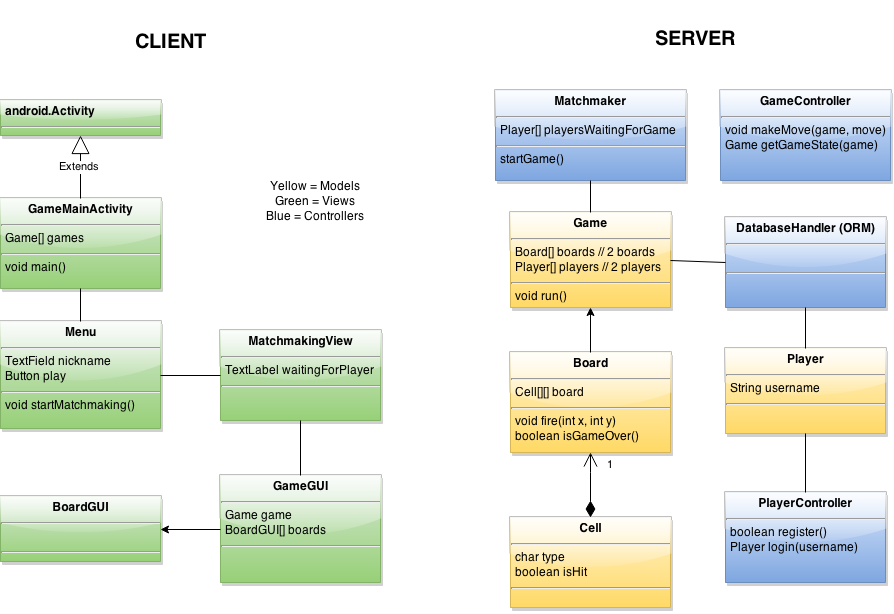
\includegraphics[width=\textwidth]{figs/class_diagram.png}
  \caption{Class Diagram for the system}
\end{figure}

\subsection{Process View}
\label{processview}

The following state diagram shows the transition between the three different views that our app consists of. You should notice that registration and login are the the same operation. The user simply writes his desired username/nickname, and clicks play. The user will then be registered in the database, if it is not there already. The user will then be able to resume his game, or start a new one if he has no ongoing games.

The Matchmaking View will be shown in the case where the current player is the only one in the Matchmaker's queue. This will probably not be a problem, as our game will be massively popular. Therefore, the MathmakerView will rarely be visible for the player.

The GameGUI will show the boards, some status text and buttons. If the game is won/lost (game over), or one of the users taps "Quit", the game is ended and the Menu will be shown again.

\begin{figure}[H]
  \centering
    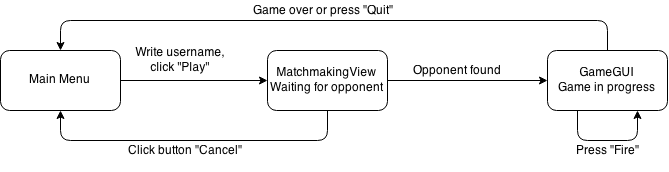
\includegraphics[width=\textwidth]{figs/state_diagram.png}
  \caption{State Diagram for the system}
\end{figure}

\begin{figure}[H]
  \centering
    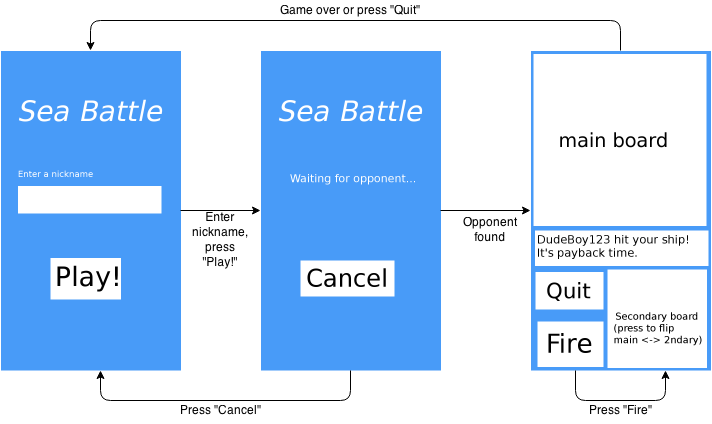
\includegraphics[width=\textwidth]{figs/gui_state_diagram.png}
  \caption{A more graphical State diagram}
\end{figure}


\begin{figure}[H]
  \centering
    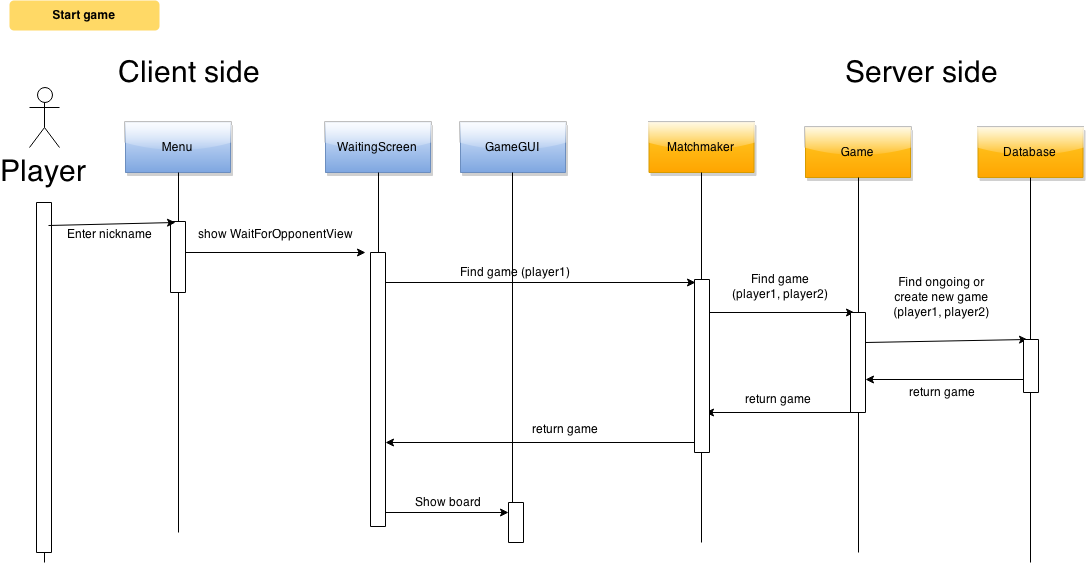
\includegraphics[width=\textwidth]{figs/sequence_diagram.png}
  \caption{Sequence Diagram for starting the system}
\end{figure}


\subsection{Development View}
\label{developmentview}

The diagram shows the main modules and components of the system. Mainly, it shows that the server (Node, Express) provides a routing-based API that the NetworkRequests module needs. The received data needs parsing on the client-side. 

Our ORM provides an interface to Express and communicates with a database.

\begin{figure}[H]
  \centering
    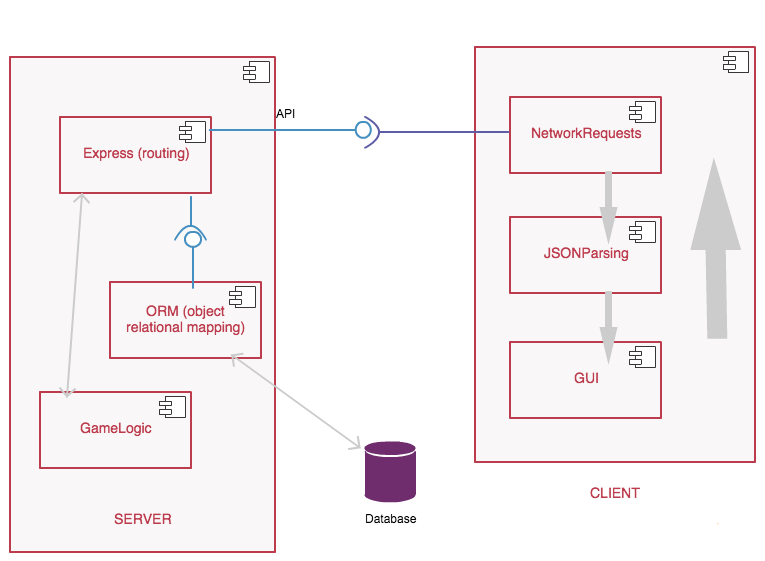
\includegraphics[width=\textwidth]{figs/component.png}
  \caption{Component Diagram for the system}
  \label{fig:component}
\end{figure}


By separating into these modules as seen in the diagram, we can split the implementation work on the group members. One could do the ORM controller (handling saving to and fetching models from the database), one could do the game logic (models and their methods), one could do the routing on the server, making sure the incoming API network requests trigger the right actions. The client side could also be separated in network handling (controller), and the different views could be delegated to different persons.

In order to make this above tactic plausible, good communication and planning are crucial factors. The database handler must know how the models are implementented to know how to store them in the database. The server network handler implementor and the client side network handler implementor must know what data to expect from each other.